\documentclass[12pt]{article}

\usepackage{polski}
\usepackage[utf8]{inputenc}
\usepackage[T1]{fontenc}
%\usepackage{indentfirst}
\usepackage{amsfonts}
\usepackage{graphicx}
\usepackage{caption}
\usepackage{multirow}
\usepackage{booktabs}
\usepackage{amssymb}
\usepackage[top=2cm, bottom=2cm, left=3cm, right=3cm]{geometry}
\usepackage{mathrsfs}
\usepackage{tikz}
\usepackage{pgfplots}
%\pagestyle{empty}
\usepackage{listings}
\usepackage{titlesec}
\usepackage{hyperref}
\usepackage{graphicx}
\usepackage{subfig}
\usepackage{natbib}
\usepackage{rotating}
\usepackage{float}

\title{\textbf{Sprawozdanie - stacja do wykrywania wyładowań atmosferycznych}\\KN EKSA}
\author{Michał Wieczorek {226284}\\ Amadeusz Wach {226379}\\ Rafał Różycki {226367} \\ Mateusz Otto {226312}}
\date{\today}

\begin{document}
\maketitle
\newpage
\section{Opis projektu}
\ Celem projektu jest konstrukcja niskobudżetowego uniwersalnego odbiornika fal krótkich o zakresie częstotliwości 3 kHz - 300 kHz. Wyładowanie atmosferyczne generuje fale elektromagnetyczne w bardzo szerokim zakresie częstotliwości. Są to impulsy, które mogą zostać odebrane ponad 1000 km od wystąpienia wyładowania. Szczegółowy teoretyczny opis zjawiska można znaleźć np. na Wikipedii. Dla częstotliwości niższych niż 100 kHz impulsy wyraźnie wybijają się ponad szum atmosferyczny, co pozwala z łatwością odebrać sygnał. Odbiornik będzie posiadać dwa wejścia na anteny ferrytowe typu H-field, co pozwoli określić przybliżoną odległość i kierunek odebranego sygnału. Anteny zostaną skonstruowane przez wykonawców projektu, ich parametry zostaną eksperymentalnie wyznaczone. Po pomyślnym zainstalowaniu odbiornika następnym krokiem będzie konstrukcja kilku następnych, co pozwoli na dokładniejsze określenie lokalizacji wystąpienia wyładowania za pomocą porównań czasów odebrania sygnału (Time of arrival method). Dane z odbiornika będą przesyłane na serwer w celu ich analizy. Projekt zakłada ukończenie prac nad jednym odbiornikiem i uruchomienie go przed końcem roku 2017. Jednym z założeń jest łatwe wprowadzanie zmian i dodatkowych modułów do odbiornika tak, aby jego użytkownicy mogli dalej go rozwijać oraz mieli możliwość prowadzenia badań. Planowane jest udostępnienie ukończonej stacji do użytku jako projekt wykonany w kole naukowym.

\section{Zrealizowane zadania i przeprowadzone testy}
\subsection{Schemat prototypu układu filtrów i wzmacniaczy skonstruowany w programie LTSpice}
\begin{figure}[H]
\begin{center}
\includegraphics[width=1\textwidth]{figures/schemat1.png}
\caption{I część Schematu układu}
\end{center}
\end{figure}
\begin{figure}[H]
\begin{center}
\includegraphics[width=1\textwidth]{figures/schemat2.png}
\caption{II część Schematu układu}
\end{center}
\end{figure}
\begin{figure}[H]
\begin{center}
\includegraphics[width=1\textwidth]{figures/ampl_faz.png}
\caption{Charakterystyka Bodego układu}
\end{center}
\end{figure}

\subsection{Skonstruowanie prototypu układu}
\begin{figure}[H]
\begin{center}
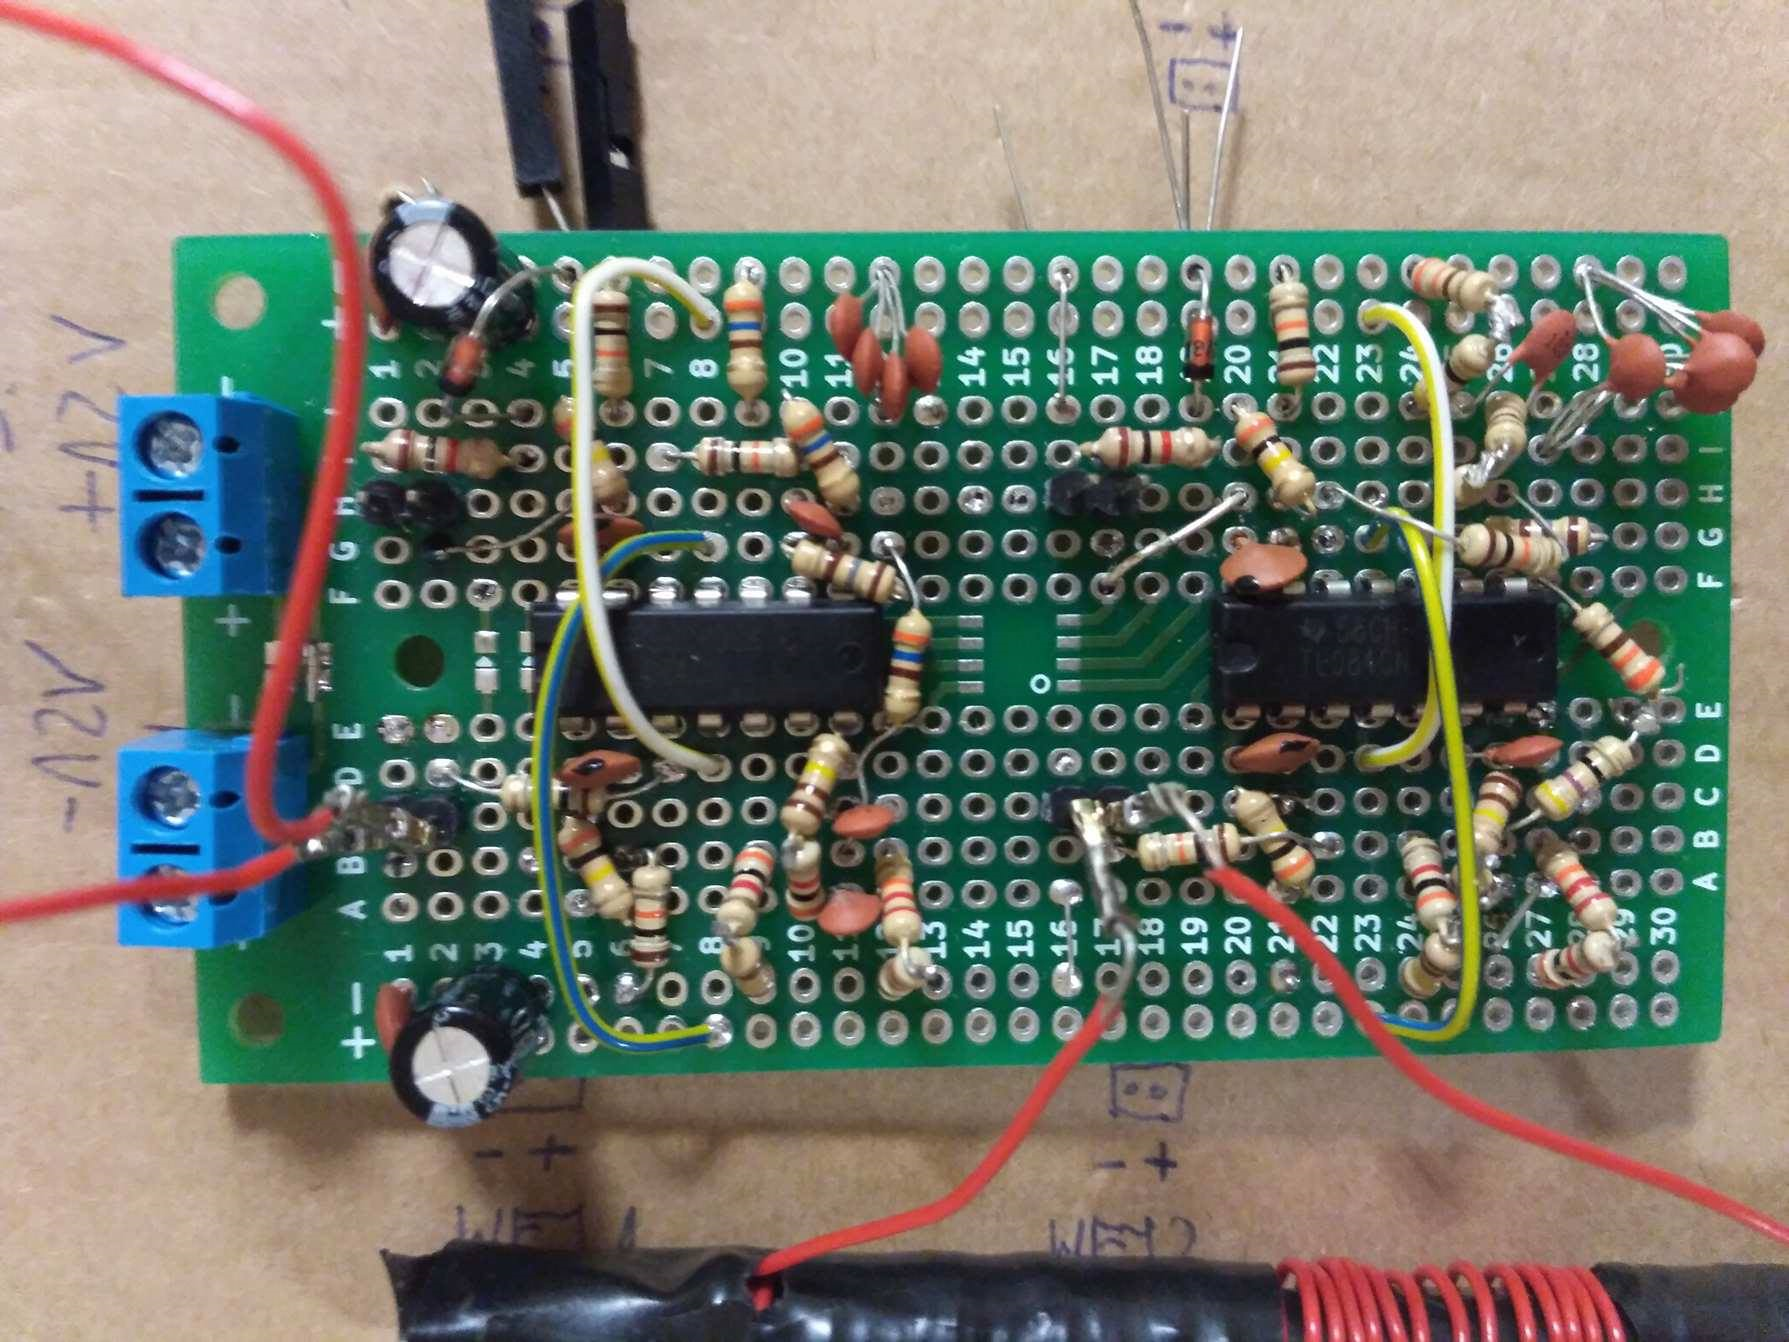
\includegraphics[width=0.95\textwidth]{figures/plytka.png}
\caption{Prototyp układu}
\end{center}
\end{figure}

\subsection{Skonstruowanie anten kierunkowych}
\ zdjęcie i podpis Anteny kierunkowe ułożone pod kątem prostym podłączone do prototypu układu\\
(Nie wiem kto ma anteny :<)

\subsection{Testy układu z wyjściem podłączonym do oscyloskopu}
\ jakieś losowe zdjęcie np. z filmu i podpis Wykrycie wyładowania atmosferycznego przez układ\\
(Amadeo tu wrzuć klatkę z nagrania bo masz w lepszej jakości)

\subsection{Próbkowanie sygnału analogowego za pomocą mikrokontrolera STM32 Nucleo}
\begin{figure}[H]
\begin{center}
\includegraphics[width=0.95\textwidth]{figures/stmstudio.png}
\caption{STMStudio - obserwacja sygnału na wyjściu układu}
\end{center}
\end{figure}
\ -zdjęcie i podpis Schemat połączeń do mikrokontrolera STM32 Nucleo (?)\\
(Amadeo tu wrzuć, najlepiej pdf na całą stronę)

\section{Kontynuacja projektu}
\ Spełnione zostały podstawowe założenia przedstawionego projektu, skonstruowano działający odbiornik poprawnie wykrywający wyładowania atmosferyczne i uniezależniono go od urządzeń laboratoryjnych (oscyloskop) za pomocą przetwornika ADC zawartego w mikrokontrolerze STM32 Nucleo. Następnym celem jest ulepszenie zestawu filtrów zawartych w układzie i praca nad modułem GPS, który odpowiedzialny będzie za zebranie informacji o bardzo dokładnym czasie wykrycia sygnału. W przyszłości zwieńczeniem projektu będzie konstrukcja kolejnych odbiorników i utworzenie sieci umożliwiającej naniesienie dokładnej lokalizacji wystąpienia na mapę. 

\end{document}